
\section{Software Design}

In order to be able to define a multilayer tree we first
designed the range and segment tree to have a template argument
defining the type of the sublayer tree. With this sublayer tree
type information the sublayers could be created. This approach lead to nested
template arguments, since the sublayer tree can again have a template
argument defining the sublayer. Therefore, the internal class and function
identifiers got longer than a compiler-dependent limit.
This happend already for $d=2$.

Therefore, we chose another, object oriented,
design. We defined  a pure
virtual base class called \ccc{Tree_base} from which we derived
the classes \ccc{Range_tree_d} and  \ccc{Segment_tree_d}.
The constructor of these classes expects an argument called
\ccc{sublayer_prototype} of type
\ccc{Tree_base}. 
Since class \ccc{Range_tree_d} and class
\ccc{Segment_tree_d} are derived from class \ccc{Tree_base}, one can
use an instantiation of class \ccc{Range_tree_d} or class
\ccc{Segment_tree_d} as constructor argument.
This argument defines the sublayer tree of the tree. E.g., you
can construct a \ccc{Range_tree_d} with an
instantiation of class \ccc{Segment_tree_d} as constructor
argument. You then have defined a range tree with a segment tree
as sublayer tree. Since both classes \ccc{Range_tree_d} and 
\ccc{Segment_tree_d} expect a sublayer tree in their constructor
we had to derive a third class called \ccc{Tree_anchor} from
class  \ccc{Tree_base} which
does not expect a constructor argument. An instantiation of this
class is used as constructor argument of class \ccc{Range_tree_d} or
\ccc{Segment_tree_d} in order to stop the recursion.

All classes provide a \ccc{clone()} function which returns an
instance (a copy) of the same tree type. The  \ccc{clone()}
function of the \ccc{sublayer_prototype} is called  in the
construction of the tree. In case that the sublayer tree again
has a sublayer, it also has a  \ccc{sublayer_prototype} which is
also cloned and so on. Thus, a call to the \ccc{clone()} function
generates a sublayer tree which has the complete knowledge about
its sublayer tree.

%Now a tree is created with a prototype of the sublayer
%tree. With this prototype the sublayer tree can be cloned. 
%More precisely, the constructor for the range and segment tree
%gets an argument called \ccc{sublayer_prototype}, which defines not
%only the type of the sublayer tree, but also the type of the
%sublayer tree
%of the sublayer tree and so on.
%Therefore, the type of this argument has to be specified. 
%This type either is of type \ccc{Range_tree_d}, \ccc{Segment_tree_d},
%or another tree data structure, that can be combined. In order to
%realize this, we made use of the OOP paradigm and defined a pure
%virtual base class called \ccc{Tree_base} from which we derived
%class \ccc{Range_tree_d} and class \ccc{Segment_tree_d}. The
%type of the constructor argument \ccc{sublayer_prototype} which
%defines the prototype is \ccc{Tree_base}.  Thus, we can assign an
%object of type \ccc{Range_tree_d} or \ccc{Segment_tree_d} to the
%variable \ccc{sublayer_prototype}. Whenever a member function of
%\ccc{sublayer_prototype} is called, the corresponding function in
%class \ccc{Range_tree_d} is called if the real type of the
%\ccc{sublayer_prototype} is \ccc{Range_tree_d}. Otherwise the
%corresponding function in class \ccc{Segment_tree_d} is called.%
%
%There is a third class derived from class \ccc{Tree_base} which
%is called \ccc{Tree_anchor}. Since the  \ccc{Range_tree_d} and
%\ccc{Segment_tree_d} classes are defined to have a sublayer tree,
%we need a sublayer which does not again have a sublayer tree, in
%order to stop the recursion. Class \ccc{Tree_anchor} plays this
%role.

%When the constructor of a \ccc{Range_tree_d} or
%\ccc{Segment_tree_d} class is called, the following happens. The
%constructor gets a prototype of its sublayer tree, which either
%is a \ccc{Range_tree_d}, 
%\ccc{Segment_tree_d}, or \ccc{Tree_anchor}. In the constructor a
%variable \ccc{sublayer_tree} is initialized with a clone of this
%prototype. Therefore, the \ccc{clone()} function of the
%prototype is called. If the prototype itself has again a sublayer
%tree, then its constructor is called with argument
%\ccc{sublayer_tree} which is the prototype of the sublayer tree
%of the prototype. This prototype is then cloned again and so on.
The
design partly follows  the {\em prototype design pattern}
in~\cite{designpatterns}. In comparison to our first approach
using templates we want to note the following: In this approach
the sublayer type is defined in
use of object oriented programming at run time, while in the
approach using templates, the sublayer type is defined at compile
time. 

The runtime overhead caused in use of virtual member
functions in this object oriented design is negligible since all virtual
functions are non trivial.
\begin{ccTexOnly}
The design concept is illustrated in Figure~\ref{rangesegmentdesign}.
\end{ccTexOnly}
\begin{ccHtmlOnly}
The design concept is illustrated in the figure below.
\end{ccHtmlOnly}

\begin{ccTexOnly}
\begin{sidewaysfigure}
%\begin{figure}[htbp]
\psfrag{A}{{\em Data}}
\psfrag{B}{{\em Window}}
\psfrag{C}{{\em Tree\_traits}}
\psfrag{D}{{\em Tree\_base$<$Data,Window$>$}}
\psfrag{E}{\small\parbox{8cm}{\em Tree\_base$<$Data,Window$>$
      *sublayer\_tree;\\
Tree\_base(Tree\_base$\&$~sublayer\_prototype);\\
Tree\_base *clone();\\
template$<$class T$>$\\
\hspace*{.2cm}virtual bool make\_tree(T$\&$~begin, T$\&$~end);\\
template$<$class T$>$\\
\hspace*{.2cm} virtual T window\_query(Window$\&$~w, T out);}}
\psfrag{F}{{\em Range\_tree\_d$<$Tree\_traits$>$}}
\psfrag{G}{\small\parbox{6cm}{\em 
Range\_tree\_d(Tree\_base$\&$~sublayer\_proto){}\\
Range\_tree\_d $\star$clone(){}\\
template$<$class T$>$\\
\hspace*{.2cm} bool make\_tree(T$\&$~begin, T$\&$~end){}\\
template$<$class T$>$\\
\hspace*{.2cm} T window\_query(Window$\&$~w, T out){}}}
\psfrag{H}{{\em Segment\_tree\_d$<$Tree\_traits$>$}}
\psfrag{I}{\small\hspace*{-.1cm}\parbox{6cm}{\em
Segment\_tree\_d(Tree\_base$\&$~slayer\_proto){}\\
Segment\_tree\_d $\star$clone(){}\\
template$<$class T$>$\\
\hspace*{.2cm} bool make\_tree(T$\&$~begin, T$\&$~end){}\\
template$<$class T$>$\\
\hspace*{.2cm} T window\_query(Window$\&$~w, T out){}}}
\psfrag{J}{{\em Tree\_anchor}}
\psfrag{K}{\small\parbox{6cm}{\em
Tree\_anchor(){}\\
Tree\_anchor $\star$clone(){}\\
template$<$class T$>$\\
\hspace*{.2cm} bool make\_tree(T$\&$~begin, T$\&$~end){}\\
template$<$class T$>$\\
\hspace*{.2cm} T window\_query(Window$\&$~w, T out){}}}
\includegraphics[width=\textwidth,clip]{rangesegmentdesign.eps}
\caption{\label{rangesegmentdesign} Design of the range and
  segment tree data structure. The symbol triangle means
that the lower class is derived from the upper class. }
%\end{figure}
\end{sidewaysfigure}
\end{ccTexOnly}

\begin{ccHtmlOnly}
    <img border=0 width=400 height=200 src="./rsd.gif" alt="Design of the range and
  segment tree data structure. The symbol triangle means
that the lower class is derived from the upper class.">
\end{ccHtmlOnly}

E.g.\ in order to define a two dimensional multilayer tree, which
consists of a range tree  in the first dimension and a segment
tree in the second dimension we proceed as follows: We construct
an object of type \ccc{Tree_anchor} which stops the
recursion. Then we construct an object of type \ccc{Segment_tree_d},
which gets as prototype argument our object of type
\ccc{Tree_anchor}. After that, we define an object of type
\ccc{Range_tree_d} which is constructed with the object of type
\ccc{Segment_tree_d} as prototype argument.
The following piece of code illustrates
the construction of the two-dimensional multilayer tree.
%This example is illustrated in Algorithm~\ref{rangesegex}.

{\small
\begin{cprog}
int main(){
  Tree_Anchor *anchor=new Tree_Anchor;
  Segment_Tree_d *segment_tree = new Segment_Tree_d(*anchor);
  Range_Tree_d *range_segment_tree = new Range_Tree_d(*segment_tree);
  /* let data_items be a list of Data items */
  range_segment_tree->make_tree(data_items.begin(),data_items.end());
}
\end{cprog}
}

Here, class \ccc{Tree_Anchor, Segment_Tree_d}, and
\ccc{Range_Tree_d} are defined by \ccc{typedef}s:

{\small
\begin{cprog}
typedef Tree_anchor<Data,Window> Tree_Anchor;
typedef Segment_tree_d<Data,Window,Interval_traits> Segment_Tree_d;
typedef Range_tree_d<Data,Window,Point_traits> Range_Tree_d;
\end{cprog}
}


%int main(){
%  Tree_anchor<Data,Window> *anchor=new Tree_anchor<Data,Window>;
%  Segment_tree_d<Data,Window,Interval_traits> *segment_tree = 
%    new Segment_tree_d<Data,Window,Interval_traits>(*anchor);
%  Range_tree_d<Data,Window,Point_traits> *range_segment_tree =
%    new Range_tree_d<Data,Window,Point_traits>(*segment_tree);
%  /* let data_items be a list of Data items */
%  range_segment_tree->make_tree(data_items.begin(),data_items.end());
%}

%The design is illustrated in
%Figure~\ref{fig:rangesegmentdesign}. 




Class \ccc{Tree\_base} and class
\ccc{Tree_anchor} get  two template arguments: a class
\ccc{Data} which defines the type of data that is stored in
the tree, and a class \ccc{Window} which defines the type of a query
range.
The derived classes \ccc{Range_tree_d} and \ccc{Segment_tree_d}
additionally get an argument called
\ccc{Tree_traits} which defines the interface between the
\ccc{Data} and the tree. Let the \ccc{Data} type be a $d$-dimensional
tuple, which is either a point data or an interval data in each
dimension. Then, the class \ccc{Tree_traits} provides accessors to
the point (resp. interval) data of that tree layer and a compare
function. Remind our example of the two-dimensional tree which
is a range tree in  the first dimension and
a segment tree  in the second dimension. Then, the
\ccc{Tree_traits} class template argument of class
\ccc{Segment_tree_d} defines an accessor to the interval data of
the \ccc{Data}, and the
\ccc{Tree_traits} class template argument of class
\ccc{Range_tree_d} defines an accessor to the point data of
\ccc{Data}.
An example implementation for these classes is listed below.
%(see Algorithm~\ref{traitsex}).

\begin{cprog}
struct Data{
  int min,max;  /* interval data */
  double point; /* point data    */
};
 
struct Window{
  int min,max;
  double min_point, max_point;
};

class Point_traits{
 public:
  typedef double Key;
  Key get_key(Data&  d){return d.point;} /*key accessor */
  Key get_left(Window& w){return w.min_point;}
  Key get_right(Window& w){return w.max_point;}
  bool comp(Key& key1, Key& key2){return (key1 < key2);} 
}

class Interval_traits{
 public:
  typedef int Key;
  Key get_left(Data&  d){return d.min;}
  Key get_right(Data&  d){return d.max;}
  Key get_left_win(Window& w){return w.min;}
  Key get_right_win(Window& w){return w.max;}
  bool comp(Key& key1, Key& key2){return (key1 < key2);} 
}
\end{cprog}



%%%%%%%%%%%%%%%%%%%%%%%%%%%%%%%%%%%%%%%%%%%%%%%%%%%%%%%%%%%%%%%%%%%%%
%%%%%%%%%%%%%%%% Predefined Trees %%%%%%%%%%%%%%%%%%%%%%%%%%%%%%%%%%
%\vfill

%\pagebreak
\section{k-dimensional Range Trees}
\label{k-range}
\cgal\ provides four range tree classes for $k\in\{1,\ldots,4\}$.

\begin{ccClassTemplate}{Range_tree_k <Traits>}

\ccDefinition

An object of the class  \ccClassName\ is a $k$-dimensional range tree
that can store k-dimensional keys of type \ccc{Key}. 
The class allows to perform
window queries on the keys.  The class \ccClassName\ is parameterized with
a range tree traits class \ccc{Traits} that defines, among other things, 
the type of the \ccc{Key}. 

\cgal\ provides traits class implementations that allow to use 
the range tree with point classes from the \cgal\ kernel as keys.
These classes are presented in Section~\ref{RT::SectPredefined}.  In
Section~\ref{RT::SectReq} we give the requirements that range tree traits
classes must fulfill. This allows the advanced user to develop further
range tree traits classes.

\ccInclude{CGAL/Range_tree_k.h}


\ccTypes

\ccNestedType{Traits}{the type of the range tree traits class.}
\ccTypedef{typedef Traits::Key Key;}{}
\ccTypedef{typedef Traits::Interval Interval;}{}

\ccCreationVariable{R}


\ccCreation

\ccConstructor{Range_tree_k ();} 
{Introduces an empty range tree \ccVar.}

\ccConstructor{template < class ForwardIterator >
               Range_tree_k (ForwardIterator first, 
                                     ForwardIterator last);}
{Introduces a range tree \ccVar\ and initializes it with the data
in the range \ccc{[first, last)}.
\ccPrecond \ccc{value_type(first) == Traits::Key}.}

\ccOperations

\ccMethod{template < class ForwardIterator >
          void 
          make_tree(ForwardIterator first,
                    ForwardIterator last);}%
{Introduces a range tree \ccVar\ and initializes it with the data
in the range \ccc{[first, last)}. This function can only be applied
once on an empty range tree.
\ccPrecond \ccc{value_type(first) == Traits::Key}.}


\ccMethod{template < class OutputIterator >
          OutputIterator
          window_query(Interval window,
                       OutputIterator out);}%
{writes all data that are in the interval \ccc{window} to the container
where \ccc{out} points to, and returns an output iterator that points
to the last location the function wrote to.
\ccPrecond  \ccc{value_type(out) == Traits::Key}.}

\end{ccClassTemplate}

\section{k-dimensional Segment Trees}
\label{segment-k}

%\subsection{CGAL\_Segment\_tree\_{\tt k} }

\label{k-segment}
\begin{ccClassTemplate}{Segment_tree_k
        <Traits>}

\ccDefinition


An object of the class  \ccClassName\ is a $k$-dimensional segment tree
that can store k-dimensional intervals  of type \ccc{Interval}. 
The class allows to perform
window queries, enclosing queries, and inverse range queries on the keys.  The class \ccClassName\ is parameterized with
a segment tree traits class \ccc{Traits} that defines, among other things, 
the type of the \ccc{Interval}. 
In order to perform an inverse range query, a range query of
$\epsilon$ width has to be performed. We prefered not to offer an
extra function for this sort of query, since the inverse range
query is a special case of the range query. Furthermore, offering
an inverse range query in the segment tree class implies offering this
function also in the range tree class and having an extra item in
the traits class that accesses the inverse range query point.


\cgal\ provides traits class implementations that allow to use 
the segment tree with point classes from the \cgal\ kernel as keys.
These classes are presented in Section~\ref{RT::SectPredefined}.  In
Section~\ref{RT::SectReq} we give the requirements that segment tree traits
classes must fulfill. This allows the advanced user to develop further
segment tree traits classes.

\ccInclude{CGAL/Segment_tree_k.h}


\ccTypes

\ccNestedType{Traits}{the type of the segment tree traits class.}
\ccTypedef{typedef Traits::Key Key;}{}
\ccTypedef{typedef Traits::Interval Interval;}{}

\ccCreationVariable{S}


\ccCreation

\ccConstructor{Segment_tree_k ();}
{Introduces an empty segment tree \ccVar.}

\ccConstructor{template < class ForwardIterator >
               Segment_tree_k (ForwardIterator first,
                                     ForwardIterator last);}%
{Introduces a segment tree \ccVar\ and initializes it with the data
in the range \ccc{[first, last)}.
\ccPrecond \ccc{value_type(first) == Traits::Interval}.}

\ccOperations

\ccMethod{template < class ForwardIterator >
          void 
          make_tree(ForwardIterator first,
                    ForwardIterator last);}%
{Introduces a segment tree \ccVar\ and initializes it with the data
in the range \ccc{[first, last)}. This function can only be applied
once on an empty segment tree.
\ccPrecond \ccc{value_type(first) == Traits::Interval}.}


\ccMethod{template < class OutputIterator >
          OutputIterator
          window_query(Interval window,
                       OutputIterator out);}%
{writes all intervals that have non empty intersection with interval \ccc{window} to the container
where \ccc{out} points to, and returns an output iterator that points
to the last location the function wrote to.
\ccPrecond  \ccc{value_type(out) == Traits::Interval}.}

\ccMethod{template < class OutputIterator >
          OutputIterator
          enclosing_query(Interval window,
                       OutputIterator out);}%
{writes all intervals that enclose in the interval \ccc{window} to the container
where \ccc{out} points to, and returns an output iterator that points
to the last location the function wrote to.
\ccPrecond  \ccc{value_type(out) == Traits::Interval}.}


\ccExample

This example illustrates the use of the predefined segment tree
on 3-dimensional interval data (with no value associated). After
the definition of the traits type and tree type, some intervals
are constructed and the tree is build according to the
intervals. Then, a window query is performed and the query
elements are given out.

\begin{cprog}
#include <CGAL/Cartesian.h>
#include <CGAL/Point_3.h>
#include <CGAL/Segment_tree_k.h>
#include <CGAL/Range_segment_tree_traits.h>

typedef CGAL::Cartesian<int> Representation;
typedef CGAL::Range_segment_tree_set_traits_3<Representation> Traits;
typedef CGAL::Segment_tree_3<Traits > Segment_tree_3_type;

int main()
{
  typedef Traits::Interval Interval;
  typedef Traits::Key Key;
  std::list<Interval> InputList, OutputList;

  InputList.push_back(Interval(Key(1,5,7), Key(2,7,9)));
  InputList.push_back(Interval(Key(2,7,6), Key(3,8,9)));
  InputList.push_back(Interval(Key(6,9,5), Key(9,13,8)));
  InputList.push_back(Interval(Key(1,3,4), Key(3,9,8)));
 
  Segment_tree_3_type Segment_tree_3(InputList.begin(),InputList.end());

  Interval a(Key(3,6,5), Key(7,12,8));
  Segment_tree_3.window_query(a,std::back_inserter(OutputList));
  std::list<Interval>::iterator j = OutputList1.begin();
  std::cout << "\n window_query (3,6,5),(7,12,8) \n";
  while(j!=OutputList.end()){
    std::cout << (*j).first.x() << "," << (*j).first.y() << ",";
    std::cout << (*j).first.z() <<", " << (*j).second.x() << ",";
    std::cout << (*j).second.y() << "," << (*j).second.z() << std::endl; 
    j++;
  }
}
\end{cprog}

\end{ccClassTemplate}


\section{Tree Traits Class Implementations  \label{RT::SectPredefined}}

This section provides range tree and segment tree traits class implementations for the
\cgal\ kernel.

\subsection{Set-like Tree Traits Classes}

The following traits classes are set-like, since no data is
associated to the keys.

\subsubsection{Set-like Tree Traits Class for 2D Kernel Points}

\begin{ccClassTemplate} {Range_segment_tree_traits_set_2<R>}

\ccDefinition
The class \ccClassName\ is a range and segment tree traits class for the
2-dimensional point class from the \cgal\ kernel. The class is
parameterized with a representation class \ccc{R}.

\ccInclude{CGAL/Range_segment_tree_traits.h}

\ccTypes
\ccTypedef{Point_2<R> Key;}{}
\ccTypedef{std::pair<Key, Key> Interval;}{}


\end{ccClassTemplate} 
\subsubsection{Set-like Tree Traits Class for 3D Kernel Points}

\begin{ccClassTemplate} {Range_segment_tree_traits_set_3<R>}

\ccDefinition
The class \ccClassName\ is a range and segment tree traits class for the 3-dimensional
point class from the \cgal\ kernel.
The class is parameterized with a representation class \ccc{R}.

\ccInclude{CGAL/Range_segment_tree_traits.h}

\ccTypes
\ccTypedef{Point_3<R> Key;}{}
\ccTypedef{std::pair<Key, Key> Interval;}{}


\end{ccClassTemplate} 


\subsection{Map-like Range Tree Traits Classes}
The following traits classes are map-like, since they allow to
associate data to the keys.


\subsubsection{Map-like Range Tree Traits Class for 2D Kernel Points}

\begin{ccClassTemplate} {Range_tree_traits_map_2<R,T>}

\ccDefinition
The class \ccClassName\ is a range tree traits class for the
2-dimensional point class from the \cgal\ kernel, where data of
type \ccc{T} is associated to each key. The class is
parameterized with a representation class \ccc{R} and the type of
the associated data \ccc{T}.

\ccInclude{CGAL/Range_segment_tree_traits.h}

\ccTypes
\ccTypedef{std::pair<Point_2<R>,T> Key;}{}
\ccTypedef{std::pair<Point_2<R>, Point_2<R> > Interval;}{}


\end{ccClassTemplate} 

\subsubsection{Map-like Range Tree Traits Class for 3D Kernel Points}

\begin{ccClassTemplate} {Range_tree_traits_map_3<R>}

\ccDefinition
The class \ccClassName\ is a range and segment tree traits class for the 3-dimensional
point class from the \cgal\ kernel,  where data of
type \ccc{T} is associated to each key.
The class is parameterized with a representation class \ccc{R} and the type of
the associated data \ccc{T}.

\ccInclude{CGAL/Range_segment_tree_traits.h}

\ccTypes
\ccTypedef{std::pair<Point_3<R>,T> Key;}{}
\ccTypedef{std::pair<Point_3<R>, Point_3<R> > Interval;}{}


\end{ccClassTemplate} 

\subsection{Map-like Segment Tree Traits Classes}
The following traits classes are map-like, since they allow to
associate data to the keys.

\subsubsection{Map-like Segment Tree Traits Class for 2D Kernel Points}

\begin{ccClassTemplate} {Segment_tree_traits_map_2<R,T>}

\ccDefinition
The class \ccClassName\ is a segment tree traits class for the
2-dimensional point class from the \cgal\ kernel, where data of
type \ccc{T} is associated to each interval. The class is
parameterized with a representation class \ccc{R} and the type of
the associated data \ccc{T}.

\ccInclude{Range_segment_tree_traits.h}

\ccTypes
\ccTypedef{Point_2<R> Key;}{}
\ccTypedef{std::pair<std::pair<Key,Key>,T> Interval;}{}


\end{ccClassTemplate} 
\subsubsection{Map-like Segment Tree Traits Class for 3D Kernel Points}

\begin{ccClassTemplate} {Segment_tree_traits_map_3<R>}

\ccDefinition
The class \ccClassName\ is a segment tree traits class for the 3-dimensional
point class from the \cgal\ kernel,  where data of
type \ccc{T} is associated to each interval.
The class is parameterized with a representation class \ccc{R} and the type of
the associated data \ccc{T}.

\ccInclude{Range_segment_tree_traits.h}

\ccTypes
\ccTypedef{std::pair<Point_3<R> > Key;}{}
\ccTypedef{std::pair<std::pair<Key, Key>,T> Interval;}{}


\end{ccClassTemplate} 

\section{ Tree Traits Class Requirements \label{RT::SectReq}}

This section describes the requirements for range and segment tree traits classes.

\begin{ccClass}{Range_segment_tree_traits_k }

\ccDefinition
A tree traits class gives the range tree and segment tree class the necessary
type information of the keys and intervals. Further more, they define function objects that allow to access
the keys and intervals, and provide comparison functions that
are needed for window queries.

\ccCreationVariable{t}
\ccTypes

\ccNestedType{Key}{The k-dimensional key type.}
\ccNestedType{Interval}{The k-dimensional interval type.}
\ccNestedType{Key_i}{The type in dimension $i$, with $1\leq i
  \leq k$.}
\ccNestedType{key_i}{function object providing an
  \ccc{operator()} that takes an argument of type \ccc{Key} and returns
  a component of type \ccc{Key_i}.}
\ccNestedType{low_i}{function object providing an
  \ccc{operator()} that takes an argument of type \ccc{Interval} and returns
  a component of type \ccc{Key_i}.}
\ccNestedType{high_i}{function object providing an
  \ccc{operator()} that takes an argument of type \ccc{Interval} and returns
  a component of type \ccc{Key_i}.}
\ccNestedType{compare_i}{function object providing an
  \ccc{operator()} that takes two arguments argument $a$, $b$ of type \ccc{Key_i} and returns
  true if $a<b$, false otherwise.}



\ccExample

The following piece of code gives an example of how a traits class
might look like, if you have keys that are of the type \ccc{int}
in the first and that are of the type \ccc{double} in the second
dimension.

\begin{cprog}
class Int_double_tree_traits_2{
 public:
  typedef std::pair<int, double> Key;
  typedef int Key_1;
  typedef double Key_2;
  typedef std::pair<Key,Key> Interval;

  class C_Key_1{
  public:
    Key_1 operator()(const Key& k)
    { return k.first;}
  };
  class C_Key_2{
  public:
    Key_2 operator()(const Key& k)
    { return k.second;}
  };
  class C_Low_1{
  public:
    Key_1 operator()(const Interval& i)
    { return i.first.first;}
  };
  class C_High_1{
  public:
    Key_1 operator()(const Interval& i)
    { return i.second.first;}
  };
  class C_Low_2{
  public:
    Key_2 operator()(const Interval& i)
    { return i.first.second;}
  };
  class C_High_2{
  public:
    Key_2 operator()(const Interval& i)
    { return i.second.second;}
  };
  class C_Compare_1{
  public:
    bool operator()(Key_1 k1, Key_1 k2)
    { return less<int>()(k1,k2);}
  };
  class C_Compare_2{
  public:
    bool operator()(Key_2 k1, Key_2 k2)
    { return less<double>()(k1,k2);}
  };
  typedef C_Compare_1 compare_1;
  typedef C_Compare_2 compare_2;
  typedef C_Low_1 low_1;
  typedef C_High_1 high_1;
  typedef C_Key_1 key_1;
  typedef C_Low_2 low_2;
  typedef C_High_2 high_2;
  typedef C_Key_2 key_2;
};
\end{cprog} 

\end{ccClass} 


\section{Creating an arbitrary multilayer tree}
\label{general}

Now let us have a closer look on how a multilayer tree is built.
In case of creating a $d$-dimensional tree,  we handle a
sequence of arbitrary data
items, where each item  defines a $d$-dimensional interval, point
or other object. The tree is constructed with an iterator over
this structure. In the $i$-th layer, the tree is
built with respect to the data slot that defines the $i$-th
dimension. Therefore, we need to define which data slot
corresponds to which dimension.
In addition we want our tree to work with arbitrary data items.
This requires an
adaptor between the algorithm and the data item. This is resolved
by the use of traits classes, implemented in
form of a traits class using
function objects.
These classes provide
access functions to a specified data slot of a data item.
A $d$-dimensional tree is then defined separately for each layer by
defining a traits class for each layer.
%Refer section~\ref{example:Segment_tree} for an example.

%%%%%%%%%%%%%%%%%%%%%%%%%%%%%%%%%%%%%%%%%%%%%%%%%%%%%%%%%%%%%%%%%%
%%%%%%%%%%%%%%%%% Interface %%%%%%%%%%%%%%%%%%%%%%%%%%%%%%%%%%%%%%
\subsection{Tree Traits class and its Requirements}
\label{TreeInterface}

Tree class \ccStyle{Range_tree_d} and class
\ccStyle{Segment_tree_d} are templatized with a parameter
\ccStyle{Traits}. \ccStyle{Traits} builds the
interface between the tree and the data items. We now describe
the traits class for a \ccStyle{Range_tree_d} layer and for a
\ccStyle{Segment_tree_d} layer. The traits classes are implemented as
template classes. If you do not want to use these traits classes you
can also define your own class which has at least to provide
the functionality of the traits class described below.


\subsubsection{tree\_point\_traits --- Requirements}

\ccDefinition
\ccStyle{tree\_point\_traits} is a template class
that provides an interface to data items.

\ccTypes
\begin{ccClass}{Point_traits}
\ccStyle{typedef}\\
\ccStyle{tree_point_traits<Data, Window, Key,
         Data_func, Window_left_func, Window_right_func,
         Compare> Point_traits;}

\ccNestedType{Data}{the container
  \ccStyle{Data} --- defines the Data type. It may consist of
         several data slots. One of these data slots has to be of
         type \ccStyle{Key}.}
\ccNestedType{Window}{the container
  \ccStyle{Window} --- defines the type of the query rectangle. It
  may consist of
         several data slots. Two of these data slots has to be of
         type \ccStyle{Key}}

\ccNestedType{Key}{the type
  \ccStyle{Key} of the data
  slot this  traits class provides access to.}

\ccNestedType{Data_func}{
  \ccStyle{Data_func} is a
         function object  providing an
  \ccc{operator()} that takes an argument of type \ccc{Data} and returns
  a component of type \ccc{Key}.}
\ccNestedType{Window_left_func}{
  \ccStyle{Window_left_func}  is a function objects that
         allow to access the
         left data slot of container
         \ccStyle{Window} which has type \ccStyle{Key}}
\ccNestedType{Window_right_func}{
  \ccStyle{Window_right_func}  is a function objects that
         allow to access the
         right data slot of container
         \ccStyle{Window} which has type \ccStyle{Key}}
\ccNestedType{Compare}{ defines a comparison relation which must
         define a strict ordering of the objects of type
         \ccStyle{Key}. If defined, \ccStyle{less<Key>}
         is sufficient.}


\ccCreation
\ccInclude{CGAL/Tree_traits.h}\\
\ccStyle{tree_point_traits<Data, Window, Key,
         Data_func, Window_left_func,
         Window_right_func, Compare> d();}\\
\ccCreationVariable{d}
%\renewcommand{\ccAlternateThreeColumn}{\ccFalse}
\hspace*{0.2\linewidth}\parbox{0.8\linewidth}{
 Generation of a \ccStyle{tree\_point\_traits} instance. It is a template class
that provides an interface to data items.}


\ccOperations
\ccMethod{Key get_key(Data d);}{The data slot of
  the data item of \ccStyle{d} of type \ccStyle{Key} is
  accessed by function object \ccStyle{Data_func}.}
\ccMethod{Key get_left(Window w);}{The data slot of
  the data item of \ccStyle{w} of type \ccStyle{Key} is
  accessed by function object
  \ccStyle{Window_left_func}.}
\ccMethod{Key get_right(Window w);}{The data slot of
  the data item of \ccStyle{w} of type \ccStyle{Key} is
  accessed by function object \ccStyle{Window_right_func}.}
\ccMethod{bool comp(Key& key1, Key&
  key2);}{returns \ccStyle{Compare(key1, key2)}.}
\ccMethod{bool key_comp(Data& data1, Data&
  data2);}{returns \ccStyle{Compare(get_key(data1), get_key(data2))}.}

\end{ccClass}

\subsubsection{tree\_interval\_traits}

\ccDefinition
\ccStyle{tree\_interval\_traits} is a template class
that provides an interface to data items. It is similar to
\ccStyle{tree\_interval\_traits}, except that it provides
access to two data slots of the same type of each container class
(\ccStyle{Data, Window}) instead of providing access to one
data slot of container class \ccStyle{Data} and two data slots
of class  \ccStyle{Window}.

\ccTypes
\begin{ccClass}{Interval_traits}
\ccStyle{typedef}\\
\ccc{tree_interval_traits<Data, Window, Key,
         Data_left_func, Data_right_func, Window_left_func,
         Window_right_func, Compare> Interval_traits;}

%\renewcommand{\ccAlternateThreeColumn}{\ccTrue}
\ccNestedType{Data}{the container \ccStyle{Data} ---
  the data type. It may consist of
         several data slots. Two of these data slots have to be of
         type \ccStyle{Key}.}
\ccNestedType{Window}{the container
  \ccStyle{Window} --- the query window type. It may consist of
         several data slots. Two of these data slots have to be of
         type \ccStyle{Key}.}
\ccNestedType{Key}{the type
  \ccStyle{Key} of the data
  slot this traits class provides access to.}
\ccNestedType{Data_left_func}{
  \ccStyle{Data_left_func} is a
         function object  providing an
  \ccc{operator()} that takes an argument of type \ccc{Data}
  and returns
  a (the left) component of type \ccc{Key}.}
\ccNestedType{Data_right_func}{
  \ccStyle{Data_right_func} is a
         function object  providing an
  \ccc{operator()} that takes an argument of type \ccc{Data}
  and returns
  a (the right) component of type \ccc{Key}.}
\ccNestedType{Window_left_func}{
  \ccStyle{Window_left_func}  is a function objects that
         allow to access the
         left data slot of container
         \ccStyle{Window} which has type \ccStyle{Key}}
\ccNestedType{Window_right_func}{
  \ccStyle{Window_right_func}  is a function objects that
         allow to access the
         right data slot of container
         \ccStyle{Window} which has type \ccStyle{Key}}
\ccNestedType{Compare}{ defines a comparison relation which must
         define a strict ordering of the objects of type
         \ccStyle{Key}. If defined, \ccStyle{less<Key>}
         is sufficient.}


\ccCreation
\ccCreationVariable{d}
\ccInclude{CGAL/Tree_traits.h}\\
%\renewcommand{\ccAlternateThreeColumn}{\ccFalse}
\ccStyle{tree_interval_traits<Data, Window, Key,
         Data_left_func, Data_right_func,
         Window_left_func,
         Window_right_func, Compare> d();}\\
\hspace*{0.2\linewidth}\parbox{0.8\linewidth}{Generation of a \ccStyle{tree\_point\_traits} instance. It is a template class
that provides an interface to data items.}

\ccOperations
\ccMethod{Key get_left(Data d);}{The data slot of
  the data item of \ccStyle{d} of type \ccStyle{Key} is
  accessed by function object
  \ccStyle{Data_left_func}.}
\ccMethod{Key get_right(Data d);}{The data slot of
  the data item of \ccStyle{d} of type \ccStyle{Key} is
  accessed by function object
  \ccStyle{Data_right_func}.}
\ccMethod{Key get_left_win(Window w);}{The data slot of
  the data item of \ccStyle{w} of type \ccStyle{Key} is
  accessed by function object
  \ccStyle{Window_left_func}.}
\ccMethod{Key get_right_win(Window w);}{The data slot of
  the data item of \ccStyle{w} of type \ccStyle{Key} is
  accessed by function object \ccStyle{Window_right_func}.}
\ccMethod{bool comp(Key& key1, Key& key2);}{returns Compare(key1, key2).}

\end{ccClass}



%%%%%%%%%%%%%%%%%%%%%%%%%%%%%%%%%%%%%%%%%%%%%%%%%%%%%%%%%%%%%%%%%%
%%%%%%%%%%%%%%%%%% Range Tree    %%%%%%%%%%%%%%%%%%%%%%%%%%%%%%%%%

%\chapter{Data Accessors and predefined Containers for Trees}
%\label{related}
%\vfill

%\pagebreak


\subsection{Range\_tree and Segment\_tree}

\ccDefinition
%The most general definition of the
%implemented range tree and segment tree is presented in this
%section.
The tree classes were first intended to have a template argument
defining the type of the sublayer tree. This leads to nested
template arguments, where the internal class and function
identifier got longer than a
compiler dependent limit. Even for dimension 2 this
happened. Therefore we chose another design. Now a tree is created
with a prototype of the sublayer tree. With this prototype the
sublayer tree can be cloned. The design pattern
corresponds to the Prototype design pattern in
~\cite{ghjv-dpero-95}.%prelim:GHVJ}.

In this sense, an instance of a
three-dimensional range tree (segment tree) would have to be
created as a range tree (segment tree) with creation variable
 \ccStyle{Sublayer\_type s}, which is a prototype of a two-dimensional
range tree (segment tree). Because a range tree or a segment tree
is expecting a prototype for its creation, a recursion anchor which
builds dimension ``zero'' is needed.
\ccStyle{Tree\_anchor} described in
section~\ref{CGALTreeanchor} fulfills all these requirements.
All tree classes (range tree, segment tree, tree anchor) are
derived from an abstract base class
\ccStyle{Tree_base}.

Additionally a range tree (segment tree) is build in function
\ccStyle{make\_tree} using  iterators.
The iterator concept is realized in the Standard
Template Library and in many other libraries,
see~\cite{ms-strg-96}. As long as the GNU, SUN and SGI compiler do not
support template member functions, we only support member
functions parameterized with iterators working on \ccStyle{STL
  list, STL vector} and \ccStyle{C-arrays}.

The trees are templatized with three arguments: \ccStyle{Data,
  Window} and \ccStyle{Traits}. Type \ccStyle{Data} defines
the input data type and type \ccStyle{Window} defines the query
window type.
The tree uses a well defined set of functions in
order to access data. These functions have to be provided by
class \ccStyle{Traits}. The requirements are described in
Section~\ref{TreeInterface}.

The trees allow to perform
window queries, enclosing queries, and inverse range queries on
the keys. Clearly, an inverse range query makes only sense in the
segment tree.
In order to perform an inverse range query, a range query of
$\epsilon$ width has to be performed. We prefered not to offer an
extra function for this sort of query, since the inverse range
query is a special case of the range query. Furthermore, offering
an inverse range query in the segment tree class implies offering this
function also in the range tree class and having an extra item in
the traits class that accesses the inverse range query point.


\begin{ccClassTemplate}{Range_tree_d<Data, Window, Traits>}
\subsubsection{Range\_tree}
\label{RangeTree}

\ccTypes
\ccNestedType{Data}{container \ccStyle{Data}.}
\ccNestedType{Window}{container \ccStyle{Window}.}
\ccNestedType{Traits}{container \ccStyle{Traits}.}

\newpage

\ccCreation
\ccCreationVariable{r}
%\renewcommand{\ccAlternateThreeColumn}{\ccFalse}
\ccInclude{CGAL/Range_tree_d.h}\\
\ccConstructor{Range_tree_d<Data, Window, Traits>
  r(Tree_base<Data, Window> sublayer_tree)}{
A range tree is
  constructed, such that the subtree of each vertex is of the
  same type prototype
\ccStyle{sublayer\_tree} is. \\
We assume that the dimension of the tree is $d$. This means, that
\ccStyle{ sublayer_tree} is a  prototype of a $d-1$-dimensional
tree. All data items of the $d$-dimensional range tree
  have container type \ccStyle{Data}. The query window of the
  tree has container type
  \ccStyle{Window}. \ccStyle{Traits}
 provides access to the corresponding data slots of container
 \ccStyle{Data} and  \ccStyle{Window} for the $d$-th
 dimension. The traits  class \ccStyle{Traits}
 must at least provide all functions and type definitions
 as described in Section~\ref{TreeInterface}.
The template class
 described there is fully generic and should fulfill the most
 requirements one can have.
In order
  to generate a one-dimensional range tree instantiate %
  \ccStyle{Tree\_anchor<Data, Window> sublayer\_tree} %
  with the same template parameters (\ccStyle{Data} and
  \ccStyle{Window}) \ccStyle{Range\_tree\_d} is defined. In
  order to construct a two-dimensional range tree, create
  \ccStyle{Range\_tree\_d} with
   a one-dimensional \ccStyle{Range\_tree\_d} with the
  corresponding \ccStyle{Traits} class of the first dimension.\\
  \ccStyle{Precondition: Traits::Data==Data and
    Traits::Window==Window.}}

\ccOperations
\ccMethod{template<class ForwardIterator>
        bool make_tree(ForwardIterator first, ForwardIterator last);}
{  The tree is constructed according to the data items in the
  sequence between the element pointed by iterator \ccStyle{first} and
  iterator \ccStyle{last}. The data items of the iterator must
  have type \ccStyle{Data}.}
\ccPrecond{This function can only be called once. If it is the
first call the tree is build and \ccStyle{true} is
returned. Otherwise, nothing is done but a \ccStyle{CGAL warning}
is given and \ccStyle{false} returned.}


\ccMethod{template<class OutputIterator>
        OutputIterator window_query(Window win, OutputIterator result);}{
   All elements that
  lay inside the  $d$-dimensional interval defined through
\ccStyle{win} are placed in the sequence container of
 \ccStyle{OutputIterator}; the output iterator that points
to the last location the function wrote to is returned.}

\ccMethod{bool is_valid();}{The tree structure is checked. For each
  vertex the subtree is checked on being valid and it is checked
  whether the value of the \ccStyle{Key_type} of a vertex
  corresponds to the highest \ccStyle{Key_type}
  value of the left subtree.}

{\bf Protected Operations}

\ccMethod{bool is_inside(Window win,
  Data object);}{returns true, if the
  data of \ccStyle{object} lies between the start and endpoint of
  interval \ccStyle{win}. False otherwise.}

\ccMethod{bool is_anchor();}{returns false.}

\ccImplementation
The construction of a $d$-dimensional range tree takes ${O}(n\log n^{d-1})$
time.  The points in
the query window are reported in time ${O}(k+{\log}^d n )$, where $k$
is the number of reported points.
The tree uses ${O}(n\log n^{d-1})$ storage.

\end{ccClassTemplate}


%%%%%%%%%%%%%%%%%%%%%%%%%%%%%%%%%%%%%%%%%%%%%%%%%%%%%%%%%%%%%%%%%%
%%%%%%%%%%%%%%%%%% Segment_tree %%%%%%%%%%%%%%%%%%%%%%%%%%%%%%%%%%%

\begin{ccClassTemplate} {Segment_tree_d<Data, Window, Traits>}
\subsubsection{Segment\_tree}
\label{SegmentTree}

\ccTypes
\ccNestedType{Data}{container \ccStyle{Data}.}
\ccNestedType{Window}{container \ccStyle{Window}.}
\ccNestedType{Traits}{class \ccStyle{Traits}.}

\ccCreation
\ccCreationVariable{s}
%\renewcommand{\ccAlternateThreeColumn}{\ccFalse}
\ccInclude{CGAL/Segment_tree_d.h}\\
\ccConstructor{Segment_tree_d<Data, Window,
  Traits> s(Tree_base<Data, Window> sublayer_tree)}%
{A segment tree is defined, such that the subtree of  each
  vertex is of the   same type prototype
\ccStyle{sublayer\_tree} is.\\
We assume that the dimension of the tree is $d$. This means, that
\ccStyle{ sublayer_tree} is a  prototype of a $d-1$-dimensional
tree. All data items of the $d$-dimensional segment tree
  have container type \ccStyle{Data}. The query window of the
  tree has container type
  \ccStyle{Window}. \ccStyle{Traits}
 provides access to the corresponding data slots of container
 \ccStyle{Data} and  \ccStyle{Window} for the $d$-th
 dimension. The traits class \ccStyle{Traits}
 must at least provide all functions and type definitions
 as described in Section~\ref{TreeInterface}.
The template class
 described there is fully generic and should fulfill the most
 requirements one can have.
In order
  to generate a one-dimensional segment tree instantiate %
  \ccStyle{Tree\_anchor<Data, Window> sublayer\_tree} %
  with the same template parameters \ccStyle{Data} and
  \ccStyle{Window} \ccStyle{Segment\_tree\_d} is defined. In
  order to construct a two-dimensional segment tree, create
  \ccStyle{Segment\_tree\_d} with
   a one-dimensional \ccStyle{Segment\_tree\_d} with the
  corresponding \ccStyle{Traits} of the first dimension.\\
  \ccStyle{Precondition: Traits::Data==Data and
    Traits::Window==Window.}}

\ccOperations
%\renewcommand{\ccAlternateThreeColumn}{\ccTrue}

\ccMethod{bool make_tree(In_it first, In_it last);}
{The tree is constructed according to the data items in the
  sequence between the element pointed by iterator \ccStyle{first} and
  iterator \ccStyle{last}.}
\ccPrecond{This function can only be called once. If it is the
first call the tree is build and \ccStyle{true} is
returned. Otherwise, nothing is done but a  \ccStyle{CGAL
  warning} is given and \ccStyle{false}
returned.}



\ccMethod{OutputIterator window_query(Window win, OutputIterator result);}
{ \ccStyle{
      win}$=[a_1,b_1),\ldots , [a_d,b_d)$, $a_i,b_i\in T_i$, $1\le
    i\le d$. All elements that
  intersect the associated $d$-dimensional interval of
\ccStyle{win} are placed in the
associated sequence container of  \ccStyle{OutputIterator}  and
returns an
output iterator that points
to the last location the function wrote to.
In order to perform an inverse range query, a range query of
$\epsilon$ width has to be performed.
}

\ccMethod{OutputIterator enclosing_query(Window win, OutputIterator result);}%
{ All elements that
  enclose the associated $d$-dimensional interval of
\ccStyle{win} are placed in the
associated sequence container of  \ccStyle{OutputIterator}  and returns an output iterator that points
to the last location the function wrote to.}

\ccMethod{bool is_valid();}{The tree structure is checked. For each
  vertex either the
  sublayer tree is a tree anchor, or it stores a (possibly empty)
  list of data items. In the first case, the sublayer tree of the
  vertex is checked on being valid. In the second case, each data
  item is checked weather it contains the associated interval of
  the vertex and does not contain the associated interval of the
  parent vertex or not. True is returned if the tree structure is valid,
  false otherwise.}

{\bf Protected Operations}

\ccMethod{bool is_inside(Window win,
  Data object);}{returns true, if the
  interval of \ccStyle{object} is contained in the
  interval of \ccStyle{win}. False otherwise.}


\ccMethod{bool is_anchor();}{returns false.}

\ccImplementation

A $d$-dimensional segment tree is constructed in ${O}(n\log n^d)$ time.
An inverse range query is performed in time ${O}(k+{\log}^d n )$, where $k$
is the number of reported intervals.
The tree uses ${O}(n\log n^d)$ storage.
\end{ccClassTemplate}


%%%%%%%%%%%%%%%%%%%%%%%%%%%%%%%%%%%%%%%%%%%%%%%%%%%%%%%%%%%%%%%%%%
%%%%%%%%%%%%%%%%%% Sub_type %%%%%%%%%%%%%%%%%%%%%%%%%%%%%%%%%%%%
\subsection{Sublayer\_type}
\label{SubtypeRequirements}
A \ccStyle{Sublayer\_type} of class \ccStyle{Range\_tree\_d}
or \ccStyle{Segment\_tree\_d} has
to fulfill the following requirements:
First of all, the class has to be derived from the abstract base
class \ccStyle{Tree_base} and therefore
has to provide  methods
\ccStyle{make\_tree}, \ccStyle{window\_query},
\ccStyle{enclosing\_query} and
\ccStyle{is\_inside}
with the same parameter types as the instantiated class
\ccStyle{Range\_tree\_d} or \ccStyle{Segment\_tree\_d},
respectively.
Furthermore a method \ccStyle{bool
  is\_anchor()} has to be provided. If the \ccStyle{Sublayer\_type} class
 builds a recursion anchor for class
\ccStyle{Segment\_tree\_d}, this function is expected to
return \ccStyle{true}, \ccStyle{false} otherwise.

Such a recursion anchor class is provided by the following class.

\begin{ccClassTemplate}{Tree_anchor<Data, Window>}
\subsubsection{Tree\_anchor}
\label{CGALTreeanchor}

\ccDefinition
\ccStyle{Tree\_anchor} is also derived from
\ccStyle{Tree\_base}. Therefore, it provides the same
methods as
\ccStyle{Range\_tree\_d} and \ccStyle{Segment\_tree\_d},
but does nothing; it can be used as a
recursion anchor for those classes. Therefore,
instantiate \ccStyle{Sublayer\_type} of \ccStyle{Range\_tree\_d}
(\ccStyle{Segment\_tree\_d} respectively)
with \ccStyle{Tree\_anchor} and the container classes for
the data items (\ccStyle{Data} and \ccStyle{Window}).


\ccCreationVariable{a}
%\renewcommand{\ccAlternateThreeColumn}{\ccFalse}

\ccDefinition
\ccNestedType{Data}{container \ccStyle{Data}.}
\ccNestedType{Window}{container \ccStyle{Window}.}

\ccCreation
\ccInclude{CGAL/Tree_base.h}

\ccConstructor{Tree_anchor<Data, Window> a()}{}
%{saves all elements in a sequence container.}

%\renewcommand{\ccAlternateThreeColumn}{\ccTrue}
\ccOperations
\ccMethod{template<class OutputIterator>
OutputIterator window_query(Window win, OutputIterator result);}{~}
%{does nothing.}
%{pushes all elements to \ccStyle{result}.}

\ccMethod{template<class OutputIterator>
OutputIterator enclosing_query(Window win, OutputIterator result);}{~}
%{does nothing.}
%{pushes all elements to \ccStyle{result}.}

\ccMethod{bool is_valid();}{returns true;}

{\bf Protected Operations}

\ccMethod{bool is_inside(Window win,
  Data object);}{returns true.}

\ccMethod{bool is_anchor();}{returns true.}



%\vfill

%\pagebreak

\ccExample
The following figures show a number of rectangles and a $2$-dimensional 
segment tree built on them.

\begin{ccTexOnly}
\begin{figure}[htbp]
%\epsfxsize=12cm
%\centerline{\epsfbox{SearchStructures/segment_ex2.eps}}
    \begin{center}
    \includegraphics[width=12cm,clip]{segment_ex2.eps}
    \end{center}
\caption{\label{fig:rectangles}Two dimensional interval data.}
\end{figure}
\begin{figure}[htbp]
%\epsfxsize=12cm
%\centerline{\epsfbox{SearchStructures/segment_ex4.eps}}
    \begin{center}
    \includegraphics[width=12cm,clip]{segment_ex4.eps}
    \end{center}
\caption{\label{fig:segTreeEx}\protect Two dimensional segment tree
  according to the interval data of Figure~\ref{fig:rectangles}.}
\end{figure}
\end{ccTexOnly}
\begin{ccHtmlOnly}
        <!2><TABLE BORDER=0 CELLSPACING=2 CELLPADDING=0 WIDTH=650>
        <TR><TD ALIGN=LEFT VALIGN=TOP WIDTH=50% NOWRAP COLSPAN=2>
  <img border=0 src="./segment_ex2.gif" alt="Two
    dimensional interval data">
 </TD><<TD WIDTH=50%></TD><TD ALIGN=LEFT VALIGN=TOP
                           NOWRAP WIDTH=50%>
 <img border=0 src="./segment_ex4.gif" alt="Two
    dimensional segment tree according to the interval data"> </TD></TR>
        </TABLE><!2>

        <!2><TABLE BORDER=0 CELLSPACING=2 CELLPADDING=0 WIDTH=650>
        <TR><TD ALIGN=LEFT VALIGN=TOP WIDTH=50% NOWRAP COLSPAN=2>
Two dimensional interval data.
 </TD><TD WIDTH=50%></TD><TD ALIGN=LEFT VALIGN=TOP WIDTH=50%>
Two dimensional segment tree
  according to the interval data.
 </TD></TR>
        </TABLE><!2>
\end{ccHtmlOnly}
\end{ccClassTemplate}

\def\ccTagRmEigenClassName{\ccTrue}
\def\ccLongParamLayout{\ccFalse}

